\begin{frame}
  \frametitle{Architecture (1)}
  \begin{center}
    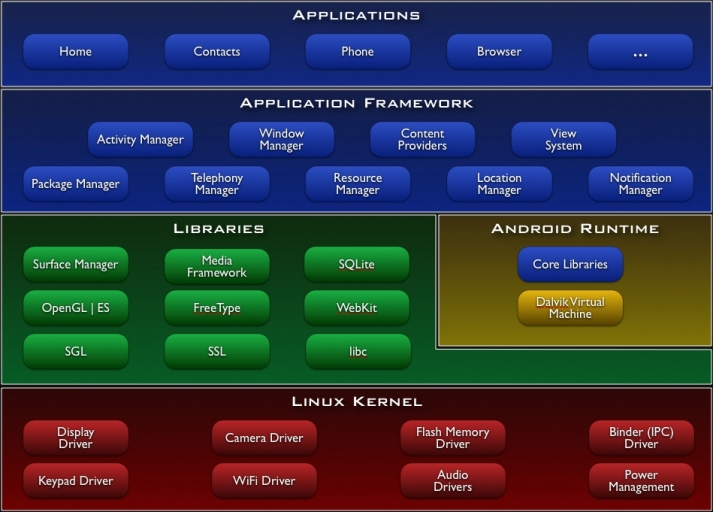
\includegraphics[height=0.8\textheight]{slides/kernel-serial-drivers-content/architecture.pdf}
  \end{center}
\end{frame}

\begin{frame}
  \frametitle{Architecture (2)}
  \begin{itemize}
  \item To be properly integrated in a Linux system, serial ports must
    be visible as TTY devices from userspace applications
  \item Therefore, the serial driver must be part of the kernel TTY
    subsystem
  \item Until 2.6, serial drivers were implemented directly behind the
    TTY core
    \begin{itemize}
    \item A lot of complexity was involved
    \end{itemize}
  \item Since 2.6, a specialized TTY driver, \code{serial_core}, eases
    the development of serial drivers
    \begin{itemize}
    \item See \code{include/linux/serial_core.h} for the main
      definitions of the \code{serial_core} infrastructure
    \end{itemize}
  \item The line discipline that cooks the data exchanged with the
    \code{tty} driver. For normal serial ports, \code{N_TTY} is used.
  \end{itemize}
\end{frame}

\begin{frame}
  \frametitle{Data Structures}
  \begin{itemize}
  \item A data structure representing a driver: \code{uart_driver}
    \begin{itemize}
    \item Single instance for each driver
    \item \code{uart_register_driver()} and
      \code{uart_unregister_driver()}
    \end{itemize}
  \item A data structure representing a port: \code{uart_port}
    \begin{itemize}
    \item One instance for each port (several per driver are possible)
    \item \code{uart_add_one_port()} and \code{uart_remove_one_port()}
    \end{itemize}
  \item A data structure containing the pointers to the operations:
    \code{uart_ops}
    \begin{itemize}
    \item Linked from \code{uart_port} through the \code{ops} field
    \end{itemize}
  \end{itemize}
\end{frame}

\begin{frame}
  \frametitle{uart\_driver}
  \begin{itemize}
  \item Usually
    \begin{itemize}
    \item Defined statically in the driver
    \item Registered in \code{module_init()}
    \item Unregistered in \code{module_cleanup()}
    \end{itemize}
  \item Contains
    \begin{itemize}
    \item \code{owner}, usually set to \code{THIS_MODULE}
    \item \code{driver_name}
    \item \code{dev_name}, the device name prefix, usually \code{ttyS}
    \item \code{major} and \code{minor}
      \begin{itemize}
      \item Use \code{TTY_MAJOR} and \code{64} to get the normal
        numbers. But they might conflict with the 8250-reserved
        numbers
      \end{itemize}
    \item \code{nr}, the maximum number of ports
    \item \code{cons}, pointer to the console device (covered later)
    \end{itemize}
  \end{itemize}
\end{frame}

\begin{frame}[fragile]
  \frametitle{uart\_driver Code Example (1)}
\begin{minted}[fontsize=\scriptsize]{c}
static struct uart_driver atmel_uart = {
    .owner = THIS_MODULE,
    .driver_name = "atmel_serial",
    .dev_name = ATMEL_DEVICENAME,
    .major = SERIAL_ATMEL_MAJOR,
    .minor = MINOR_START,
    .nr = ATMEL_MAX_UART,
    .cons = ATMEL_CONSOLE_DEVICE,
};

static struct platform_driver atmel_serial_driver = {
    .probe = atmel_serial_probe,
    .remove = atmel_serial_remove,
    .suspend = atmel_serial_suspend,
    .resume = atmel_serial_resume,
    .driver = {
        .name = "atmel_usart",
        .owner = THIS_MODULE,
    },
};
\end{minted}
Example code from \code{drivers/serial/atmel_serial.c}
\end{frame}

\begin{frame}[fragile]
  \frametitle{uart\_driver Code Example (2)}
\begin{minted}[fontsize=\small]{c}
static int __init atmel_serial_init(void)
{
    /* Warning: Error management removed */
    uart_register_driver(&atmel_uart);
    platform_driver_register(&atmel_serial_driver);
    return 0;
}

static void __exit atmel_serial_exit(void)
{
    platform_driver_unregister(&atmel_serial_driver);
    uart_unregister_driver(&atmel_uart);
}

module_init(atmel_serial_init);
module_exit(atmel_serial_exit);
\end{minted}
\end{frame}

\begin{frame}
  \frametitle{uart\_port}
  \begin{itemize}
  \item Can be allocated statically or dynamically
  \item Usually registered at \code{probe()} time and unregistered at
    \code{remove()} time
  \item Most important fields
    \begin{itemize}
    \item \code{iotype}, type of I/O access, usually \code{UPIO_MEM}
      for memory-mapped devices
    \item \code{mapbase}, physical address of the registers
    \item \code{irq}, the IRQ channel number
    \item \code{membase}, the virtual address of the registers
    \item \code{uartclk}, the clock rate
    \item \code{ops}, pointer to the operations
    \item \code{dev}, pointer to the device (\code{platform_device}
      or other)
    \end{itemize}
  \end{itemize}
\end{frame}

\begin{frame}[fragile]
  \frametitle{uart\_port Code Example (1)}
\begin{minted}[fontsize=\tiny]{c}
static int atmel_serial_probe(struct platform_device *pdev)
{
    struct atmel_uart_port *port;

    port = &atmel_ports[pdev->id];
    port->backup_imr = 0;

    atmel_init_port(port, pdev);

    uart_add_one_port(&atmel_uart, &port->uart);

    platform_set_drvdata(pdev, port);

    return 0;
}

static int atmel_serial_remove(struct platform_device *pdev)
{
    struct uart_port *port = platform_get_drvdata(pdev);

    platform_set_drvdata(pdev, NULL);
    uart_remove_one_port(&atmel_uart, port);

    return 0;
}
\end{minted}
\end{frame}

\begin{frame}[fragile]
\frametitle{uart\_port Code Example (2)}
\begin{minted}[fontsize=\footnotesize]{c}
static void atmel_init_port(
    struct atmel_uart_port *atmel_port,
    struct platform_device *pdev)
{
    struct uart_port *port = &atmelt_port->uart;
    struct atmel_uart_data *data = pdev->dev.platform_data;

    port->iotype = UPIO_MEM;
    port->flags = UPF_BOOT_AUTOCONF;
    port->ops = &atmel_pops;
    port->fifosize = 1;
    port->line = pdev->id;
    port->dev = &pdev->dev;

    port->mapbase = pdev->resource[0].start;
    port->irq = pdev->resource[1].start;

    tasklet_init(&atmel_port->tasklet, atmel_tasklet_func,
        (unsigned long)port);

\end{minted}
\end{frame}

\begin{frame}[fragile]
\frametitle{uart\_port Code Example (3)}
\begin{minted}[fontsize=\footnotesize]{c}
    if (data->regs)
        /* Already mapped by setup code */
        port->membase = data->regs;
    else {
        port->flags |= UPF_IOREMAP;
        port->membase = NULL;
    }

    /* for console, the clock could already be configured */
    if (!atmel_port->clk) {
        atmel_port->clk = clk_get(&pdev->dev, "usart");
        clk_enable(atmel_port->clk);
        port->uartclk = clk_get_rate(atmel_port->clk);
        clk_disable(atmel_port->clk);
        /* only enable clock when USART is in use */
    }
}
\end{minted}
\end{frame}

\begin{frame}
  \frametitle{uart\_ops}
  \begin{itemize}
  \item Important operations
    \begin{itemize}
    \item \code{tx_empty()}, tells whether the transmission FIFO is
      empty or not
    \item \code{set_mctrl()} and \code{get_mctrl()}, allow to set and
      get the modem control parameters (RTS, DTR, LOOP, etc.)
    \item \code{start_tx()} and \code{stop_tx()}, to start and stop
      the transmission
    \item \code{stop_rx()}, to stop the reception
    \item \code{startup()} and \code{shutdown()}, called when the port
      is opened/closed
    \item \code{request_port()} and \code{release_port()},
      request/release I/O or memory regions
    \item \code{set_termios()}, change port parameters
    \end{itemize}
  \item See the detailed description in
    \kerneldoc{serial/driver}
  \end{itemize}
\end{frame}

\begin{frame}[fragile]
  \frametitle{Implementing Transmission}
  \begin{itemize}
  \item The \code{start_tx()} method should start transmitting
    characters over the serial port
  \item The characters to transmit are stored in a circular buffer,
    implemented by a \code{struct uart_circ} structure. It contains
    \begin{itemize}
    \item \code{buf[]}, the buffer of characters
    \item \code{tail}, the index of the next character to
      transmit. After transmit, tail must be updated using
      \mint{c}+tail = tail &(UART_XMIT_SIZE - 1)+
    \end{itemize}
  \item Utility functions on \code{uart_circ}
    \begin{itemize}
    \item \code{uart_circ_empty()}, tells whether the circular buffer
      is empty
    \item \code{uart_circ_chars_pending()}, returns the number of
      characters left to transmit
    \end{itemize}
  \item From an \code{uart_port} pointer, this structure can be
    reached using \code{port->state->xmit}
  \end{itemize}
\end{frame}

\begin{frame}[fragile]
  \frametitle{Polled-Mode Transmission}
\begin{minted}[fontsize=\footnotesize]{c}
foo_uart_putc(struct uart_port *port, unsigned char c) {
    while(__raw_readl(port->membase + UART_REG1) & UART_TX_FULL)
        cpu_relax();
    __raw_writel(c, port->membase + UART_REG2);
}

foo_uart_start_tx(struct uart_port *port) {
    struct circ_buf *xmit = &port->state->xmit;

    while (!uart_circ_empty(xmit)) {
        foo_uart_putc(port, xmit->buf[xmit->tail]);
        xmit->tail = (xmit->tail + 1) & (UART_XMIT_SIZE - 1);
        port->icount.tx++;
    }
}
\end{minted}
\end{frame}

\begin{frame}[fragile]
  \frametitle{Transmission with Interrupts (1)}
\begin{minted}{c}
foo_uart_interrupt(int irq, void *dev_id) {
    [...]
    if (interrupt_cause & END_OF_TRANSMISSION)
        foo_uart_handle_transmit(port);
    [...]
}

foo_uart_start_tx(struct uart_port *port) {
    enable_interrupt_on_txrdy();
}
\end{minted}
\end{frame}

\begin{frame}[fragile]
\frametitle{Transmission with Interrupts (2)}
\begin{minted}[fontsize=\footnotesize]{c}
foo_uart_handle_transmit(port) {
    struct circ_buf *xmit = &port->state->xmit;
    if (uart_circ_empty(xmit) || uart_tx_stopped(port)) {
        disable_interrupt_on_txrdy();
        return;
    }

    while (!uart_circ_empty(xmit)) {
        if (!(__raw_readl(port->membase + UART_REG1) &
            UART_TX_FULL))
            break;
        __raw_writel(xmit->buf[xmit->tail],
            port->membase + UART_REG2);
        xmit->tail = (xmit->tail + 1) & (UART_XMIT_SIZE - 1);
        port->icount.tx++;
    }

    if (uart_circ_chars_pending(xmit) < WAKEUP_CHARS)
        uart_write_wakeup(port);
}
\end{minted}
\end{frame}

\begin{frame}
  \frametitle{Reception}
  \begin{itemize}
  \item On reception, usually in an interrupt handler, the driver must
    \begin{itemize}
    \item Increment \code{port->icount.rx}
    \item Call \code{uart_handle_break()} if a \code{BRK} has been
      received, and if it returns TRUE, skip to the next character
    \item If an error occurred, increment \code{port->icount.parity},
      \code{port->icount.frame}, \code{port->icount.overrun} depending
      on the error type
    \item Call \code{uart_handle_sysrq_char()} with the received
      character, and if it returns TRUE, skip to the next character
    \item Call \code{uart_insert_char()} with the received character
      and a status
      \begin{itemize}
      \item Status is \code{TTY_NORMAL} is everything is OK, or
        \code{TTY_BREAK}, \code{TTY_PARITY}, \code{TTY_FRAME} in case
        of error
      \end{itemize}
    \item Call \code{tty_flip_buffer_push()} to push data to the TTY
      layer
    \end{itemize}
  \end{itemize}
\end{frame}

\begin{frame}
  \frametitle{Understanding Sysrq}
  \begin{itemize}
  \item Part of the reception work is dedicated to handling
    \code{Sysrq}
    \begin{itemize}
    \item Sysrq are special commands that can be sent to the kernel to
      make it reboot, unmount filesystems, dump the task state, nice
      real-time tasks, etc.
    \item These commands are implemented at the lowest possible level
      so that even if the system is locked, you can recover it.
    \item Through serial port: send a \code{BRK} character, send the
      character of the \code{Sysrq} command
    \item See \kerneldoc{sysrq.txt}
    \end{itemize}
  \item In the driver
    \begin{itemize}
    \item \code{uart_handle_break()} saves the current time + 5
      seconds in a variable
    \item \code{uart_handle_sysrq_char()} will test if the current
      time is below the saved time, and if so, will trigger the
      execution of the Sysrq command
    \end{itemize}
  \end{itemize}
\end{frame}

\begin{frame}[fragile]
  \frametitle{Reception Code Sample (1)}
\begin{minted}[fontsize=\scriptsize]{c}
foo_receive_chars(struct uart_port *port) {
    int limit = 256;

    while (limit-- > 0) {
        status = __raw_readl(port->membase + REG_STATUS);
        ch = __raw_readl(port->membase + REG_DATA);
        flag = TTY_NORMAL;

        if (status & BREAK) {
            port->icount.break++;
            if (uart_handle_break(port))
                continue;
        }
        else if (status & PARITY)
            port->icount.parity++;
        else if (status & FRAME)
            port->icount.frame++;
        else if (status & OVERRUN)
            port->icount.overrun++;

        [...]
\end{minted}
\end{frame}

\begin{frame}[fragile]
\frametitle{Reception Code Sample (2)}
\begin{minted}[fontsize=\scriptsize]{c}
        [...]
        status &= port->read_status_mask;

        if (status & BREAK)
            flag = TTY_BREAK;
        else if (status & PARITY)
            flag = TTY_PARITY;
        else if (status & FRAME)
            flag = TTY_FRAME;

        if (uart_handle_sysrq_char(port, ch))
            continue;

        uart_insert_char(port, status, OVERRUN, ch, flag);
    }

    spin_unlock(& port->lock);
    tty_flip_buffer_push(port->state->port.tty);
    spin_lock(& port->lock);
}
\end{minted}
\end{frame}

\begin{frame}
  \frametitle{Modem Control Lines}
  \begin{itemize}
  \item Set using the \code{set_mctrl()} operation
    \begin{itemize}
    \item The \code{mctrl} argument can be a mask of \code{TIOCM_RTS}
      (request to send), \code{TIOCM_DTR} (Data Terminal Ready),
      \code{TIOCM_OUT1}, \code{TIOCM_OUT2}, \code{TIOCM_LOOP} (enable
      loop mode)
    \item If a bit is set in \code{mctrl}, the signal must be driven
      active, if the bit is cleared, the signal must be driven
      inactive
    \end{itemize}
  \item Status using the \code{get_mctrl()} operation
    \begin{itemize}
    \item Must return read hardware status and return a combination of
      \code{TIOCM_CD} (Carrier Detect), \code{TIOCM_CTS} (Clear to
      Send), \code{TIOCM_DSR} (Data Set Ready) and \code{TIOCM_RI}
      (Ring Indicator)
    \end{itemize}
  \end{itemize}
\end{frame}

\begin{frame}[fragile]
  \frametitle{set\_mctrl() Example}
\begin{minted}[fontsize=\scriptsize]{c}
foo_set_mctrl(struct uart_port *uart, u_int mctrl) {
    unsigned int control = 0, mode = 0;

    if (mctrl & TIOCM_RTS)
        control |= ATMEL_US_RTSEN;
    else
        control |= ATMEL_US_RTSDIS;

    if (mctrl & TIOCM_DTS)
        control |= ATMEL_US_DTREN;
    else
        control |= ATMEL_US_DTRDIS;

    __raw_writel(port->membase + REG_CTRL, control);

    if (mctrl & TIOCM_LOOP)
        mode |= ATMEL_US_CHMODE_LOC_LOOP;
    else
        mode |= ATMEL_US_CHMODE_NORMAL;

    __raw_writel(port->membase + REG_MODE, mode);
}
\end{minted}
\end{frame}

\begin{frame}[fragile]
\frametitle{get\_mctrl() example}
\begin{minted}[fontsize=\footnotesize]{c}
foo_get_mctrl(struct uart_port *uart, u_int mctrl) {
    unsigned int status, ret = 0;

    status = __raw_readl(port->membase + REG_STATUS);

    /*
     * The control signals are active low.
     */
     if (!(status & ATMEL_US_DCD))
         ret |= TIOCM_CD;
     if (!(status & ATMEL_US_CTS))
         ret |= TIOCM_CTS;
     if (!(status & ATMEL_US_DSR))
         ret |= TIOCM_DSR;
     if (!(status & ATMEL_US_RI))
         ret |= TIOCM_RI;

     return ret;
}
\end{minted}
\end{frame}

\begin{frame}
  \frametitle{termios}
  \begin{itemize}
  \item \emph{The termios functions describe a general terminal
      interface that is provided to control asynchronous
      communication ports}
  \item A mechanism to control from userspace serial port parameters
    such as
    \begin{itemize}
    \item Speed
    \item Parity
    \item Byte size
    \item Stop bit
    \item Hardware handshake
    \item Etc.
    \end{itemize}
  \item See \code{termios(3)} for details
  \end{itemize}
\end{frame}

\begin{frame}[fragile]
  \frametitle{set\_termios()}
  \begin{itemize}
  \item The \code{set_termios()} operation must
    \begin{itemize}
    \item apply configuration changes according to the arguments
    \item update \code{port->read_config_mask} and
      \code{port->ignore_config_mask} to indicate the events we are
      interested in receiving
    \end{itemize}
  \item \mint{c}+static void set_termios(struct uart_port *port,+
    \mint{c}+struct ktermios *termios, struct ktermios *old)+
    \begin{itemize}
    \item \code{port}, the port, \code{termios}, the new values and
      \code{old}, the old values
    \end{itemize}
  \item Relevant \code{ktermios} structure fields are
    \begin{itemize}
    \item \code{c_cflag} with word size, stop bits, parity, reception
      enable, CTS status change reporting, enable modem status change
      reporting
    \item \code{c_iflag} with frame and parity errors reporting, break
      event reporting
    \end{itemize}
  \end{itemize}
\end{frame}

\begin{frame}[fragile]
  \frametitle{set\_termios() example (1)}
\begin{minted}[fontsize=\scriptsize]{c}
static void atmel_set_termios(struct uart_port *port,
    struct ktermios *termios, struct ktermios *old)
{
    unsigned long flags;
    unsigned int mode, imr, quot, baud;

    mode = __raw_readl(port->membase + REG_MODE);
    baud = uart_get_baud_rate(port, termios, old, 0, port->uartclk / 16);
    /* Read current configuration */
    quot = uart_get_divisor(port, baud);

    /* Compute the mode modification for the byte size parameter */
    switch (termios->c_cflag & CSIZE) {
    case CS5:
        mode |= ATMEL_US_CHRL_5;
        break;
    case CS6:
        mode |= ATMEL_US_CHRL_6;
        break;
    [...]
    default:
        mode |= ATMEL_US_CHRL_8;
        break;
    }
\end{minted}
\end{frame}

\begin{frame}[fragile]
  \frametitle{set\_termios() example (2)}
\begin{minted}[fontsize=\scriptsize]{c}
    /* Compute the mode modification for the stop bit */
    if (termios->c_cflag & CSTOPB)
        mode |= ATMEL_US_NBSTOP_2;

    /* Compute the mode modification for parity */
    if (termios->c_cflag & PARENB) {
        /* Mark or Space parity */
        if (termios->c_cflag & CMSPAR) {
            if (termios->c_cflag & PARODD)
                mode |= ATMEL_US_PAR_MARK;
            else
                mode |= ATMEL_US_PAR_SPACE;
        } else if (termios->c_cflag & PARODD)
            mode |= ATMEL_US_PAR_ODD;
        else
            mode |= ATMEL_US_PAR_EVEN;
    } else
        mode |= ATMEL_US_PAR_NONE;

    /* Compute the mode modification for CTS reporting */
    if (termios->c_cflag & CRTSCTS)
        mode |= ATMEL_US_USMODE_HWHS;
    else
        mode |= ATMEL_US_USMODE_NORMAL;
\end{minted}
\end{frame}

\begin{frame}[fragile]
  \frametitle{set\_termios() Example (3)}
\begin{minted}[fontsize=\scriptsize]{c}
    /* Compute the read_status_mask and ignore_status_mask 
     * according to the events we're interested in. These
     * values are used in the interrupt handler. */
    port->read_status_mask = ATMEL_US_OVRE;
    if (termios->c_iflag & INPCK)
        port->read_status_mask |= (ATMEL_US_FRAME | ATMEL_US_PARE);
    if (termios->c_iflag & (BRKINT | PARMRK))
        port->read_status_mask |= ATMEL_US_RXBRK;

    port->ignore_status_mask = 0;
    if (termios->c_iflag & IGNPAR)
        port->ignore_status_mask |= (ATMEL_US_FRAME | ATMEL_US_PARE);
    if (termios->c_iflag & IGNBRK) {
        port->ignore_status_mask |= ATMEL_US_RXBRK;
        if (termios->c_iflag & IGNPAR)
            port->ignore_status_mask |= ATMEL_US_OVRE;
    }
    /* The serial_core maintains a timeout that corresponds to the
     * duration it takes to send the full transmit FIFO. This timeout has
     * to be updated. */
    uart_update_timeout(port, termios->c_cflag, baud);
\end{minted}
\end{frame}

\begin{frame}[fragile]
  \frametitle{set\_termios() Example (4)}
\begin{minted}[fontsize=\scriptsize]{c}
    /* Finally, apply the mode and baud rate modifications. Interrupts,
     * transmission and reception are disabled when the modifications
     * are made. */

    /* Save and disable interrupts */
    imr = UART_GET_IMR(port);
    UART_PUT_IDR(port, -1);
    /* disable receiver and transmitter */
    UART_PUT_CR(port, ATMEL_US_TXDIS | ATMEL_US_RXDIS);
    /* set the parity, stop bits and data size */
    UART_PUT_MR(port, mode);
    /* set the baud rate */
    UART_PUT_BRGR(port, quot);
    UART_PUT_CR(port, ATMEL_US_RSTSTA | ATMEL_US_RSTRX);
    UART_PUT_CR(port, ATMEL_US_TXEN | ATMEL_US_RXEN);
    /* restore interrupts */
    UART_PUT_IER(port, imr);
    /* CTS flow-control and modem-status interrupts */
    if (UART_ENABLE_MS(port, termios->c_cflag))
        port->ops->enable_ms(port);
}
  \end{minted}
\end{frame}

\begin{frame}
  \frametitle{Console}
  \begin{itemize}
  \item To allows early boot messages to be printed, the kernel
    provides a separate but related facility: \code{console}
    \begin{itemize}
    \item This console can be enabled using the \code{console=} kernel
      argument
    \end{itemize}
  \item The driver developer must
    \begin{itemize}
    \item Implement a \code{console_write()} operation, called to
      print characters on the console
    \item Implement a \code{console_setup()} operation, called to
      parse the \code{console=} argument
    \item Declare a \code{struct console} structure
    \item Register the console using a \code{console_initcall()}
      function
    \end{itemize}
  \end{itemize}
\end{frame}

\begin{frame}[fragile]
  \frametitle{Console: Registration}
\begin{minted}[fontsize=\scriptsize]{c}
static struct console serial_txx9_console = {
    .name = TXX9_TTY_NAME,
    .write = serial_txx9_console_write,
    /* Helper function from the serial_core layer */
    .device = uart_console_device,
    .setup = serial_txx9_console_setup,
    /* Ask for the kernel messages buffered during
     * boot to be printed to the console when activated */
    .flags = CON_PRINTBUFFER,
    .index = -1,
    .data = &serial_txx9_reg,
};

static int __init serial_txx9_console_init(void)
{
    register_console(&serial_txx9_console);
    return 0;
}

/* This will make sure the function is called early during the boot process.
 * start_kernel() calls console_init() that calls our function */
console_initcall(serial_txx9_console_init);
\end{minted}
\end{frame}

\begin{frame}[fragile]
  \frametitle{Console: Setup}
\begin{minted}[fontsize=\tiny]{c}
static int __init serial_txx9_console_setup(struct console *co,
    char *options)
{
    struct uart_port *port;
    struct uart_txx9_port *up;
    int baud = 9600;
    int bits = 8;
    int parity = 'n';
    int flow = 'n';

    if (co->index >= UART_NR)
        co->index = 0;
    up = &serial_txx9_ports[co->index];
    port = &up->port;
    if (!port->ops)
        return -ENODEV;

    /* Function shared with the normal serial driver */
    serial_txx9_initialize(&up->port);
    
    if (options)
        /* Helper function from serial_core that parses the console= string */
        uart_parse_options(options, &baud, &parity, &bits, &flow);

    /* Helper function from serial_core that calls the ->set_termios() */
    /* operation with the proper arguments to configure the port */
    return uart_set_options(port, co, baud, parity, bits, flow);
}
\end{minted}
\end{frame}

\begin{frame}[fragile]
  \frametitle{Console: Write}
\begin{minted}[fontsize=\tiny]{c}
static void serial_txx9_console_putchar(struct uart_port *port, int ch)
{
	struct uart_txx9_port *up = (struct uart_txx9_port *)port;
	/* Busy-wait for transmitter ready and output a single character. */
	wait_for_xmitr(up);
	sio_out(up, TXX9_SITFIFO, ch);
}

static void serial_txx9_console_write(struct console *co,
    const char *s, unsigned int count)
{
    struct uart_txx9_port *up = &serial_txx9_ports[co->index];
    unsigned int ier, flcr;
	
    /* Disable interrupts */
    ier = sio_in(up, TXX9_SIDICR);
    sio_out(up, TXX9_SIDICR, 0);
   
    /* Disable flow control */
    flcr = sio_in(up, TXX9_SIFLCR);
    if (!(up->port.flags & UPF_CONS_FLOW) && (flcr & TXX9_SIFLCR_TES))
        sio_out(up, TXX9_SIFLCR, flcr & ~TXX9_SIFLCR_TES);

    /* Helper function from serial_core that repeatedly calls the given putchar() */
    /* callback */
    uart_console_write(&up->port, s, count, serial_txx9_console_putchar);
	
    /* Re-enable interrupts */
    wait_for_xmitr(up);
    sio_out(up, TXX9_SIFLCR, flcr);
    sio_out(up, TXX9_SIDICR, ier);
}
\end{minted}
\end{frame}
